\clearpage

\section{ゲームを\ruby{改造}{かい|ぞう}してみよう}
\subsection{ドロップパズルの改造}

ファイル→「開く」メニューから/home/ユーザー名/02のフォルダに移動してから、「drop.hsp」を読み込んでみましょう。

\begin{figure}[H]
    \begin{center}
        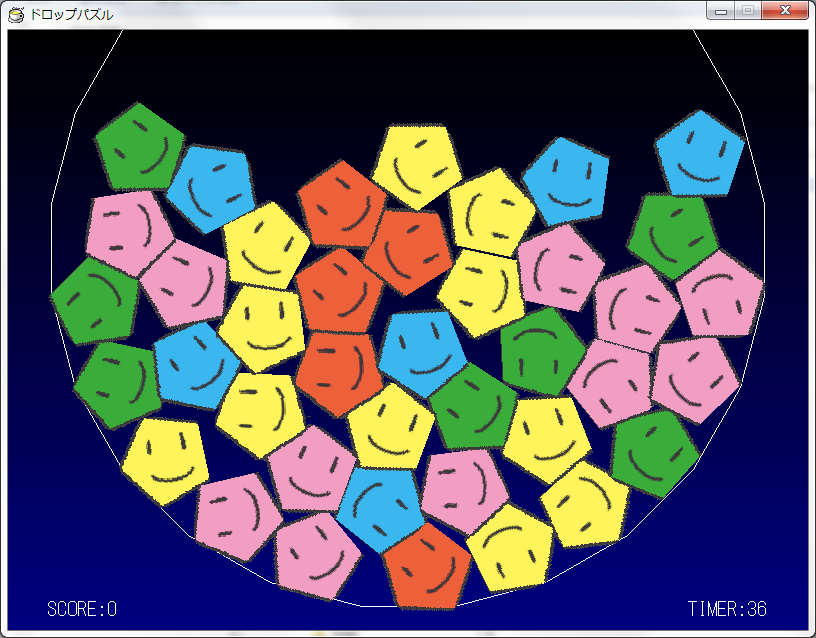
\includegraphics[keepaspectratio,width=8.356cm,height=6.544cm]{text02-img/text02-img015.png}
        \caption{ドロップパズルゲームの画面}
    \end{center}
\end{figure}

ドロップパズルゲームを改造して、自分だけのゲームに変えてみます。
スクリプトは、簡単に修正できることを学びました。実は、ゲームの中の絵も自由に修正することができます。

\subsection{GIMPを使ってみよう}

ここでは、第1回で使ったRaspberry Piで絵を描くためのプログラム「GIMP」を使ってみます。
ファイルマネージャーの画面から、「/home/ユーザー名/02」フォルダにある「koma.png」のアイコンで右クリックを押して、「GIMP ( GNU Image Manipulation Program )」のメニューを選ぶすることでツールを起動させることができます。
これで、「koma.png」を読み込んで下絵とすることができます。

\begin{figure}[H]
    \begin{center}
        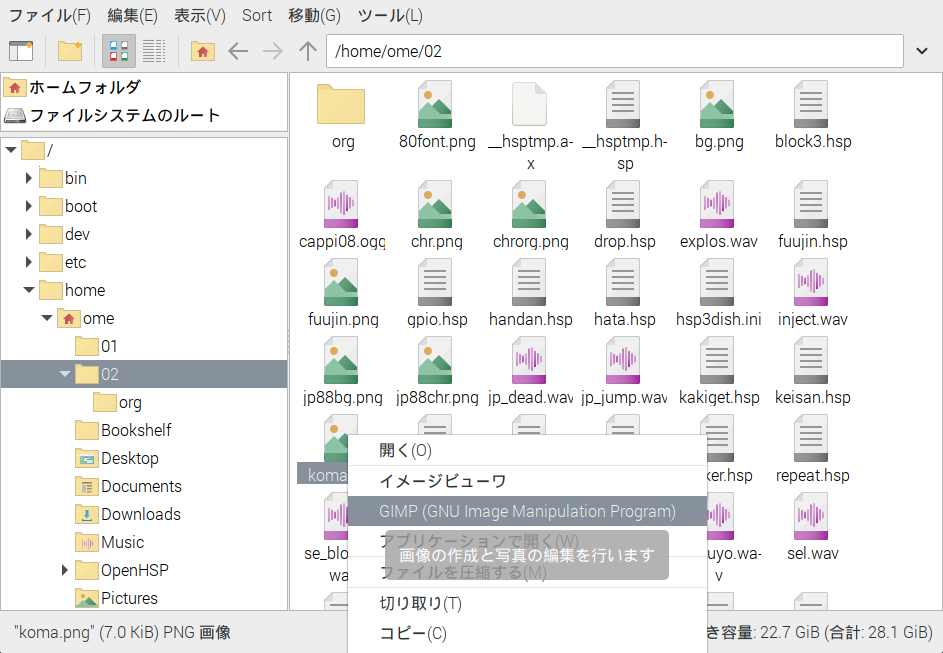
\includegraphics[keepaspectratio,width=10.583cm,height=7.938cm]{text02-img/s_komapng.png}
        \caption{koma.pngからGIMPを起動するところ}
    \end{center}
\end{figure}

\subsection{ドロップパズルの中身を変えてみよう}

GIMPを使って、ドロップパズルのゲームで使われた絵を改造してみましょう。
GIMPは、絵のデータを読み込んで、自分で好きに変更することができます。
変更した絵は、ふたたび保存することができます。

\begin{figure}[H]
    \begin{center}
        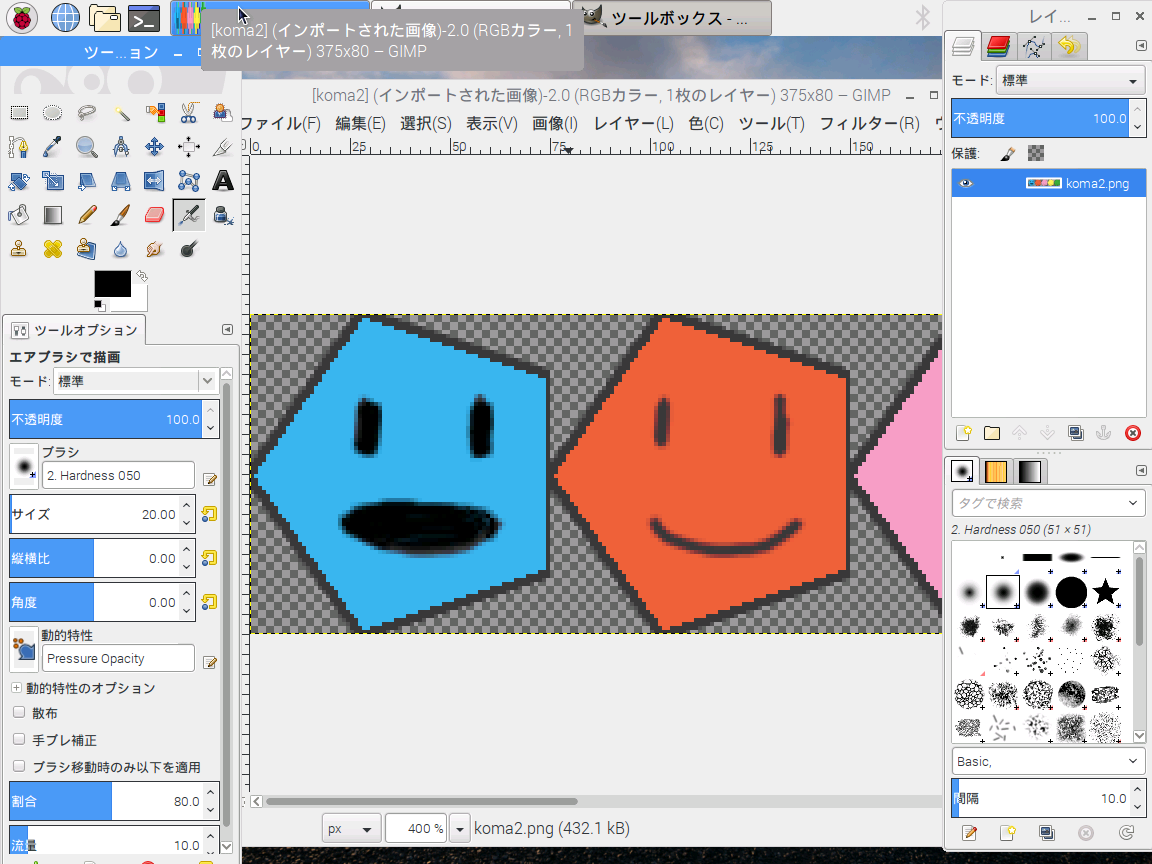
\includegraphics[keepaspectratio,width=10.403cm,height=7.811cm]{text02-img/text02-img038.png}
        \caption{koma.pngを修正している画面}
    \end{center}
\end{figure}

このキャラクターを\ruby{別}{べつ}な絵に書き\ruby{換}{か}えればゲームの絵も変わります。
パレットで色を選んで、\ruby{鉛筆}{えん|ぴつ}のツールで絵を書いていきます。
元の絵があった部分を書き換えて他の\ruby{絵柄}{え|がら}にしてみましょう。

\begin{figure}[H]
    \begin{center}
        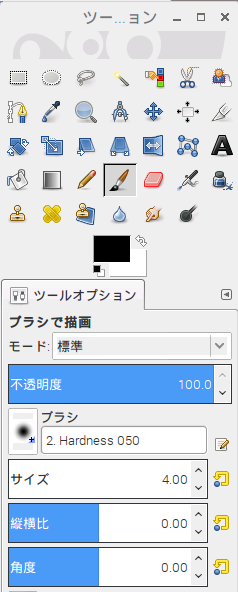
\includegraphics[keepaspectratio,width=4.075cm,height=10.16cm]{text02-img/text02-img039.png}
        \caption{ツールのウインドウ}
    \end{center}
\end{figure}

画像が小さい場合は、画像の下にある「100\%」の右側にあるボタンを押して、「400\%」「800\%」などを選ぶと\ruby{拡大}{かく|だい}されます。
絵を修正する時には、ツールアイコンの中から「ブラシ」を選択して、サイズを4〜6くらいの数字に変えてから絵の上で、マウスボタンを押しながら動かして色を置きます。

色を\ruby{変更}{へん|こう}する場合は、ツールパレットの\ruby{描画色}{びょう|が|しょく}をクリックして、「描画色の変更」ダイアログを出してから好きな色を選びます。

\begin{figure}[H]
    \begin{center}
        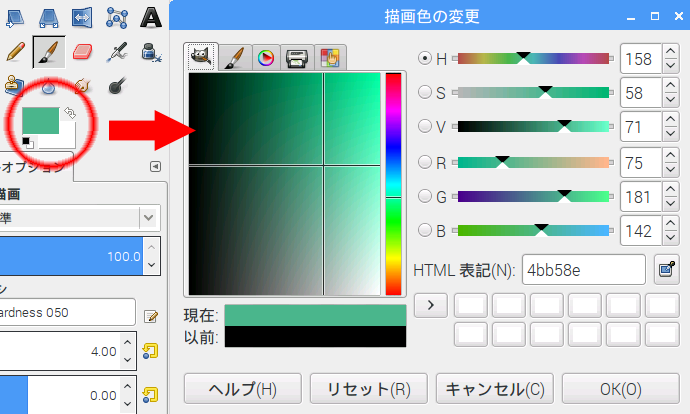
\includegraphics[keepaspectratio,width=10.993cm,height=6.588cm]{text02-img/text02-img040.png}
        \caption{色をえらぶところ}
    \end{center}
\end{figure}

元の絵を書き換えたら、ファイル→「koma.pngに上書きエクスポート」を選んで保存します。
作業が終わったら、最後にファイル→「終了」を選んでGIMPアプリケーションを閉じるのを忘れないでください。
通常の「保存」メニューを選択すると元のPNGファイルではなく、GIMP専用のファイル形式でて保存されてしまいます。
今回は、PNGファイルだけを保存したいので、「koma.pngに上書きエクスポート」を選んで保存するようにしてください。

変更した画像でゲームを動かしてみましょう。
HSPスクリプトエディタを起動して、「drop.hsp」を読み込みます。
[F5]キーを押して実行して変わっていれば成功です。

本当にスクリプトからゲームが作られているのか確かめてみましょう。
たとえば、ドロップパズルゲームのスクリプトには、「name=”ドロップパズル”」と書かれている部分があります。

\begin{figure}[H]
    \begin{center}
        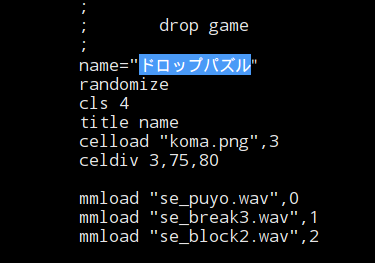
\includegraphics[keepaspectratio,width=9.049cm,height=6.346cm]{text02-img/text02-img014.png}
        \caption{ドロップパズルのスクリプト}
    \end{center}
\end{figure}

これを、「name=”ドロドロパズル”」など他の文字に変えてみてください。
[F5]キーで実行して、どこが変わっているか確認してみましょう。

「k=rnd(5)」という部分を探してみましょう。
これは106行目にあります。カーソルがある行の数は左下に「line:〇〇〇」表示されていますので確認してみましょう )
この「5」を「3」などもっと少ない数に変えてみるとどうなるか確認してみましょう。

\begin{figure}[H]
    \begin{center}
        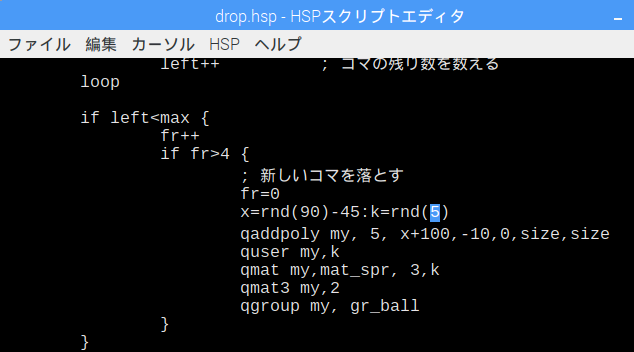
\includegraphics[keepaspectratio,width=12.753cm,height=7.064cm]{text02-img/text02-img041.png}
    \end{center}
\end{figure}

変更したスクリプトは、ファイル→「\ruby{上書}{うわ|が}き保存」によりdrop.hspに保存することができます。
別な名前で保存したい時には、ファイル→「名前を付けて保存…」で新しいファイルとして保存することができます。
これから先、さらに色々な部分を変えてみながら、プログラムの動きについて覚えていきましょう。

これで、あなたが改造したオリジナルのパズルゲームになりました。

\subsection{例題に挑戦しよう}

ここまで終わってしまった人は、以下の例題にも挑戦してみよう。

\begin{itemize}
    \item シューティングゲーム(shoot)の絵を改造する
    \item シューティングゲーム(shoot)のスクリプトを改造する
    \item タイトルを変えてみよう
    \item 敵や味方の強さを変えてみよう
    \item ゲーム全体の速さを変えてみよう
\end{itemize}

例題の考え方がわからない時は、近くのTAか先生に聞いてください。
わからない所は、そのままにせず、必ず答えを見つけてから先に進みましょう。